\begin{figure}[!ht]
 \centering
 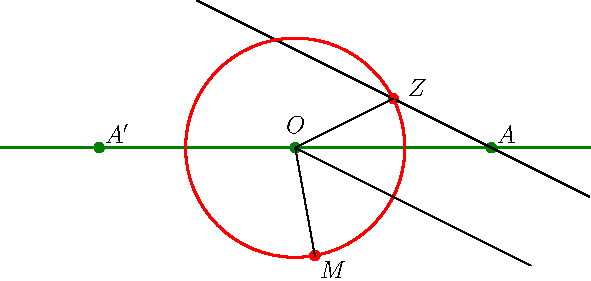
\includegraphics{Ccomp8_1.pdf}
 \caption{Bissectrice $(OZ),(OM)$}
 \label{fig:Ccomp8_1}
\end{figure}

\begin{enumerate}
 \item Comme $a$ est réel, $\overline{z}-a$ est le conjugué de $z-a$. Ils ont donc le même module ce qui entraine que $|m| = |\overline{z}|=|z|$. Donc $OM=OZ$ et $M$ et $Z$ sont sur un même cercle de centre $O$. 
 \item Notons $\alpha$ un argument de $z-a$ et $\theta$ un argument de $z$. Alors $e^{i\alpha}$ est l'affixe d'un vecteur directeur de $AZ$ et $e^{i\theta}$ est l'affixe d'un vecteur directeur de $(O,Z)$. De plus on peut écrire
\begin{displaymath}
 m = |z|e^{i(2\alpha - \theta)}
\end{displaymath}
Le complexe $e^{i(2\alpha - \theta)}$ est donc l'affixe d'un vecteur directeur de $(O,M)$. Notons $\mu = 2\alpha -\theta$, c'est un argument de ce vecteur directeur. On a alors
\begin{displaymath}
 \alpha = \frac{1}{2}(\theta + \mu)
\end{displaymath}
ce qui montre que $(AZ)$ est la bissectrice des demi-droites $(OM)$ et $(OZ)$.

\begin{figure}[!ht]
 \centering
 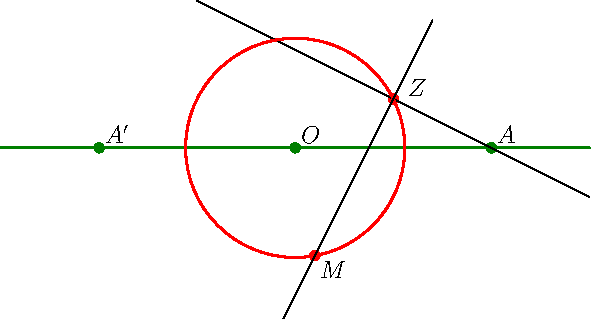
\includegraphics{Ccomp8_2.pdf}
 \caption{Construction du point $M$}
 \label{fig:Ccomp8_2}
\end{figure}

 \item On calcule en utilisant la définition :
\[
 m-z = \overline{z}\,\frac{z-a}{\overline{z}-a}-z
=\frac{|z|^2 - a\overline{z} -|z|^2 + az}{\overline{z}-a}
=\frac{2ia \Im(z)}{\overline{z}-a}
\Rightarrow
\frac{m-z}{z-a}=\frac{2ia \Im(z)}{|\overline{z}-a|^2}
\]
De manière analogue:
\begin{displaymath}
 m+a = \overline{z}\,\frac{z-a}{\overline{z}-a} +a
= \frac{|z|^2 - a\overline{z} +\overline{z}a -a^2}{\overline{z}-a}=\frac{|z|^2-a^2}{\overline{z}-a}
\end{displaymath}
En divisant par la relation précédente, on obtient bien:
\begin{displaymath}
 \frac{m+a}{m-z} = i\,\frac{a^2-|z|^2}{2a\Im z}
\end{displaymath}
On en déduit que la droite $(MZ)$ est orthogonale aux droites $(AZ)$ et à $(MA')$. Les droites $(AZ)$ et $(MA')$ sont parallèles car toutes les deux orthogonales à $(ZM)$.\newline
On construit géométriquement $M$ en prenant le point d'intersection de la droite perpendiculaire à $(AZ)$ en $A$ avec le cercle de centre $O$ qui passe par $Z$.. 
\end{enumerate}
